\usepackage[authoryear,round]{natbib}
\usepackage{multirow}
\usetikzlibrary{decorations.pathmorphing}

\newcommand{\sheetnum}{%
	01
}
%\setcounter{section}{\sheetnum-3}
\newcommand{\tutorialtitle}{%
    Principal Component Analysis
}
\newcommand{\tutorialtitleshort}{%
	PCA
}
% for slides
\subtitle{\sheetnum \tutorialtitle}

\maxdeadcycles=1000 % Workaround for ! Output loop---100 consecutive dead cycles because of too many figures

% The following use of algroithms is recommended for the notes:
%
%\begin{figure}[!t]
%\removelatexerror
%\begin{algorithm}[H]
    % your algo here
    %\label{alg:algolabel}
    %\caption{algocaption}
%\end{algorithm}
%\end{figure}
%\begin{algorithm}
% Below is the definition for the command \removelatexerror:
\makeatletter
\newcommand{\removelatexerror}{\let\@latex@error\@gobble}
\makeatother

\begin{document} %%%%%%%%%%%%%%%%%%%%%%%%%%%%%%%%%%%%%%%%%%%%%%%%%%%%%%%

\sheet{\sheetnum}{\tutorialtitleshort}

\ttopic{\tutorialtitle}

\begin{frame}
    \titlepage
\end{frame}

\begin{frame}
    \tableofcontents[subsubsectionstyle=hide]
\end{frame}

\newpage

\columnratio{0.2,0.8}\textbf{}
\begin{paracol}{2}
%\setlength{\columnseprule}{0.1pt}
%\setlength{\columnsep}{5em}

\begin{rightcolumn}

\mode<all>
\section{The setting}

\begin{frame}\frametitle{\secname}
    
\underline{Data:}

observations: $\big\{ \vec{x}^{(\alpha)} \big\}, \alpha = 1, \ldots, p; \quad \vec{x} \in \R^N$

$$
\vec x = \rmat{
x_1\\
x_2\\
\vdots\;\,\\
x_N
}
$$

Our entire dataset:
\[
\vec X = 
\left(
\begin{array}{cccc}
\Big| & \Big| & &\Big| \\[3mm]
\vec x^{(1)} & \vec x^{(2)} & \cdots &\vec x^{(p)}\\[2mm]
\Big| & \Big| & &\Big|
\end{array}
\right) \in \R^{N \times p}
\]

\end{frame}

\section{Dimensionality Reduction}

\begin{frame}\frametitle{\secname}
We want to reduce the number of elements in $\vec x \in \R^N$
while retaining most of the intrinsic information content.

\question{For what purpose?}\\

\question{What is the difference between dimensionality reduction and compression, if any?}

\end{frame}

%\newpage
\subsection{Simple truncation}

\begin{frame}\frametitle{\subsecname}

\begin{center}
\begin{minipage}{0.3\textwidth}

	%\begin{table}[]
	%\centering
	\resizebox{\textwidth}{!}{%
	\begin{tabular}{c|cccc}
			  & \multicolumn{1}{c}{$\vec x^{(1)}$} & \multicolumn{1}{c}{$\vec x^{(2)}$} & \multicolumn{1}{c}{\ldots} & $\vec x^{(p)}$ \\ \hline%\cline{1-3} \cline{5-5} 
	$x_1$     & -0.2                           & 0.1                            &                       & 0.2       \\ \cline{1-1}
	$x_2$     & 0.1                            & 3.1                            &                       & -1.0      \\ \cline{1-1}
	$x_3$     & 2.5                            & 7.2                            &                       & -0.8      \\ %\cline{1-1}
	  \vdots        &            \vdots                    &     \vdots                          & \begin{tabular}[c]{@{}c@{}}\ldots\vspace{2.5mm}\end{tabular} &      \vdots     \\ %\cline{1-1}
	$x_{N-2}$ & -7.1                           & -3.5                           &                       & 7.0       \\ \cline{1-1}
	$x_{N-1}$ & -10.3                          & -0.3                           &                       & 4.5       \\ \cline{1-1}
	$x_N$     & 4.0                            & 1.3                            &                       & 6.6       \\ \hline
	\end{tabular}%
	}
	%\end{table}
\end{minipage}
\begin{minipage}{\slidesonly{0.33}\notesonly{0.15}\textwidth}
	\begin{center}
		\includegraphics[width=0.99\textwidth]{img/telephone_masts_depth}%
	\end{center}
\end{minipage}
\begin{minipage}{0.3\textwidth}

	\resizebox{\textwidth}{!}{%
	\begin{tabular}{c|cccc}
	\only<-3>{		  & \multicolumn{1}{c}{$\vec{{ x}}^{(1)}$} & \multicolumn{1}{c}{$\vec{{ x}}^{(2)}$} & \multicolumn{1}{c}{\ldots} & $\vec{{ x}}^{(p)}$ \\ \hline%\cline{1-3} \cline{5-5} 
	}
	\only<4->{		  & \multicolumn{1}{c}{$\vec{{\widetilde x}}^{(1)}$} & \multicolumn{1}{c}{$\vec{{\widetilde x}}^{(2)}$} & \multicolumn{1}{c}{\ldots} & $\vec{{\widetilde x}}^{(p)}$ \\ \hline%\cline{1-3} \cline{5-5} 
	}
	$ x_1$     & -0.2                           & 0.1                            &                       & 0.2       \\ \cline{1-1}
	$ x_2$     & 0.1                            & 3.1                            &                       & -1.0      \\ \cline{1-1}
	$ x_3$     & 2.5                            & 7.2                            &                       & -0.8      \\ %\cline{1-1}
	  \vdots        &            \vdots                    &     \vdots                          & \begin{tabular}[c]{@{}c@{}}\ldots\vspace{2.5mm}\end{tabular} &      \vdots     \\ %\cline{1-1}
	$ x_{N-2}$ & -7.1                           & -3.5                           &                       & 7.0       \\ \cline{1-1}
	\slidesonly{
	\only<1>{
	$ x_{N-1}$ & -10.3                          & -0.3                           &                       & 4.5       \\ \cline{1-1}
	$ x_N$     & 4.0                            & 1.3                            &                       & 6.6       \\ \hline
	}
	\only<3>{
	%\hline{\vspace{\dimexpr 2.2ex-\doublerulesep}}
	$\hcancel[red]{{{ x}}_{N-1}}$ &          \textcolor{red}{?}             &          \textcolor{red}{?}             &                    &    \textcolor{red}{?}   \\ \cline{1-1}
	$\hcancel[red]{{{ x}}_{N}}$     &                      \textcolor{red}{?}        &               \textcolor{red}{?}            &                   & \textcolor{red}{?}      \\ \hline
	}
	}
	\only<4->{
	%\hline{\vspace{\dimexpr 2.2ex-\doublerulesep}}
	$\color{blue}{{{\widetilde x}}_{N-1}}$ &          \textcolor{blue}{0}             &          \textcolor{blue}{0}          &                    &   \textcolor{blue}{0}  \\ \cline{1-1}
	$\color{blue}{{{\widetilde x}}_{N}}$     &                      \textcolor{blue}{0}        &              \textcolor{blue}{0}           &                   & \textcolor{blue}{0}   \\ \hline
	}
	\end{tabular}%
	}
\end{minipage}

\only<2>{
\mode<presentation>{
	\begin{center}
		\includegraphics[width=0.2\textwidth]{img/telegram}
		\captionof*{figure}{\tiny
		Photo by \href{https://unsplash.com/@sandratansh?utm_source=unsplash&utm_medium=referral&utm_content=creditCopyText}{Sandra Tan} on \href{https://unsplash.com/s/photos/telegram?utm_source=unsplash&utm_medium=referral&utm_content=creditCopyText}{Unsplash}
	}%
	\end{center}
	}
}
\only<5>{
\vspace{5mm}
	restore $N$-dimensional vector using \textcolor{blue}{zero padding}.
	
\svspace{5mm}

\begin{minipage}{.8\textwidth}
\begin{minipage}{0.33\textwidth}
	\begin{center}
		\includegraphics[width=0.99\textwidth]{img/tram}%
	\end{center}
\end{minipage}
\hfill
\begin{minipage}{0.33\textwidth}
	\begin{center}
		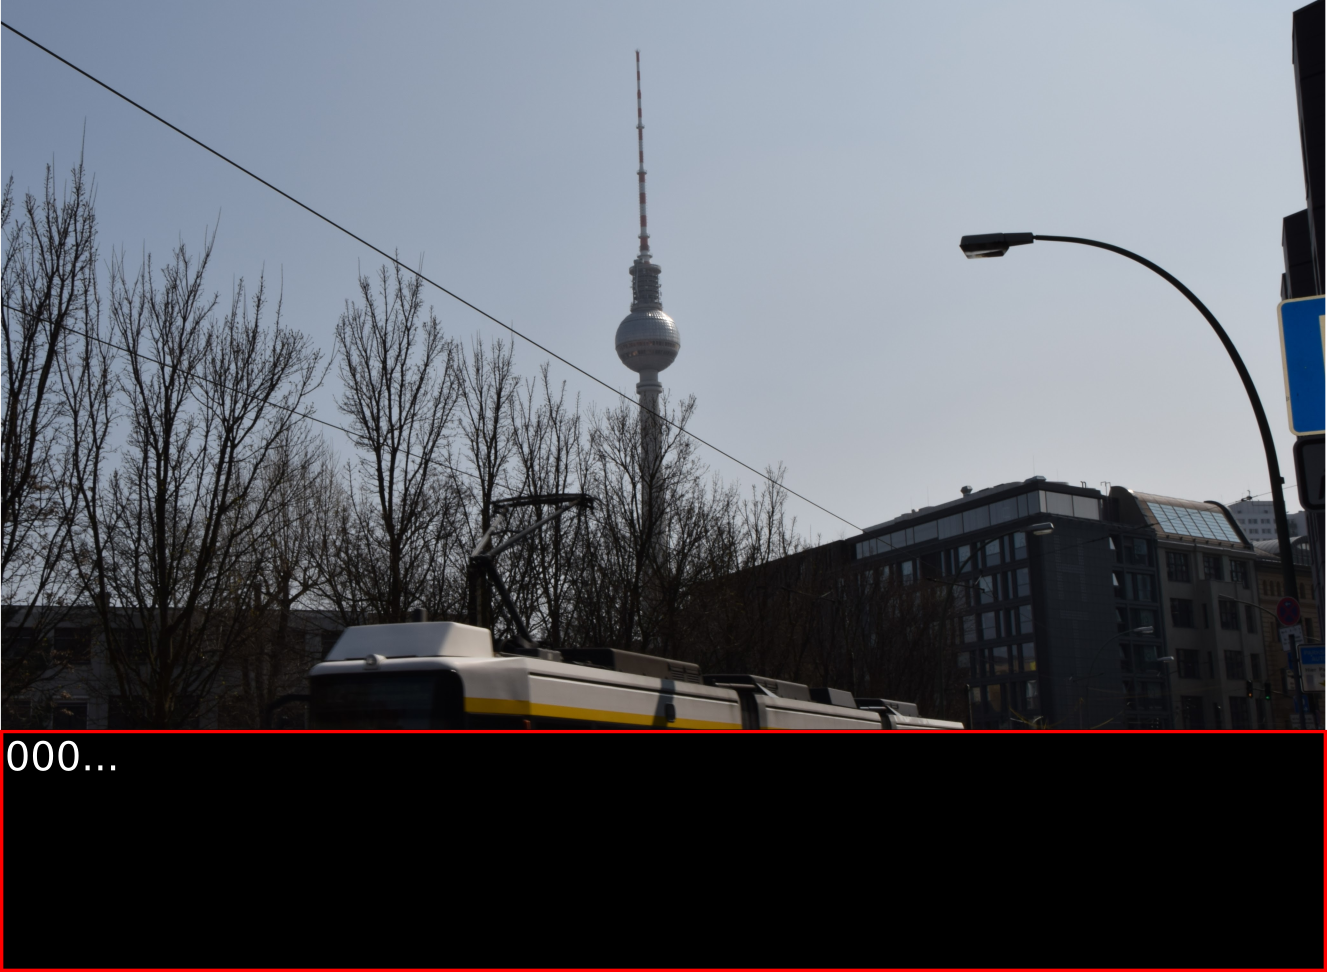
\includegraphics[width=0.99\textwidth]{img/tram_missing_box}%
	\end{center}
\end{minipage}
\end{minipage}
}



\end{center}

\end{frame}

\subsubsection{Procedure}

\begin{frame}\frametitle{\subsecname:~\subsubsecname}

Let
\svspace{-5mm}
\begin{itemize}
\item[]$\vec x \in \R^N$,\\
\item[] w.l.o.g. $\E[\vec x] \eqexcl \vec 0$ \notesonly{\\

}, i.e. for each variable $x_i$ its mean $m_i = \sum_{\alpha=1}^{p} x_i^{(\alpha)} \eqexcl 0$.
\end{itemize}

\pause

\begin{enumerate}
\item \underline{Dimensionality Reduction}: From $N$ to $\color{red}M$ with $0 < {\color{red}M}\, < N$\\
$\Rightarrow$ simply transmit the first $\color{red}M$ elements of $\vec x$. 
\pause
\item \underline{Reconstruction}: The recipient reconstructs all $N$ elements by adding zero entries for all missing elements (i.e. \textit{zero-padding}):\\
Let $\widetilde{\vec{x}}$ be the reconstructed observation, where\\ 
 
 \begin{equation}
 % = $ for $j=1,\ldots,M% (perfect reconstruction for the first $M$ elements),
 \widetilde{x}_j = \begin{cases} 
      {x}_j & \text{for}~j=1,\ldots,{\color{red}M} \qquad \text{(perfect reconstruction)} \\
      0 & \text{for}~j={\color{red}M}+1,\ldots,N \quad \text{zero-padding} 
   \end{cases}
 \end{equation}
\end{enumerate}

\question{How much error will the recipient accumulate in the case of simple truncation?}

\end{frame}

\subsubsection{Measuring the error}\label{sec:objective}

\begin{frame}\frametitle{\subsecname:~\subsubsecname}

\notesonly{
We measure the MSE between every original point $\vec x$ and its reconstruction $\widetilde{\vec{x}}$.

Let $\widetilde{\vec{x}}$ be the reconstructed observation. }

\slidesonly{\vspace{-7mm}}

\begin{align}
\label{eq:mse}
\visible<1->{
\mathit{MSE}  &=  \frac{1}{p} \sum\limits_{\alpha = 1}^p ( \vec{x}^{(\alpha)} - \widetilde{\vec{x}}^{(\alpha)} )^2
	\notesonly{\\&}=  \frac{1}{p} \sum\limits_{\alpha = 1}^p \sum\limits_{j = 1}^N ( {x}_j^{(\alpha)} - {\widetilde{{x}}}^{(\alpha)}_j )^2\\
	\intertext{The \textcolor{red}{first $M$} elements were transmitted perfectly, \textcolor{blue}{zero padding} is used to extend the vector to its original size of $N$ elements}
}
\visible<2->{
     &=  \frac{1}{p} \sum\limits_{\alpha = 1}^p \bigg(
     \underbrace{
		{\color{red}\sum\limits_{j = 1}^M} ( x_j^{(\alpha)} - \widetilde{x}_j^{(\alpha)} )^2
		}_{
		\substack{=0 \\\text{ (perfect transmission)}}
		} 
		+ {\color{blue}\sum\limits_{j = M+1}^N} ( x_j^{(\alpha)} - 
	\underbrace{
	\vphantom{\sum\limits_{j = 1}^M ( x_j^{(\alpha)} - \widetilde{x}_j^{(\alpha)} )^2}
	\widetilde{x}_j^{(\alpha)}
	}_{\substack{=0\\ \text{padded}}}
	\kern-0.5ex)^2 \bigg)\\
     &=  \frac{1}{p} \sum\limits_{\alpha = 1}^p {\color{blue}\sum\limits_{j = M+1}^N} ( x_j^{(\alpha)} )^2
     \slidesonly{\;\;}\notesonly{\\&}=  {\color{blue}\sum\limits_{j = M+1}^N} \frac{1}{p} \sum\limits_{\alpha = 1}^p  ( x_j^{(\alpha)} )^2 \\
     &=  {\color{blue}\sum\limits_{j = M+1}^N} \sigma_j^2
     }
\end{align}

\end{frame}

\begin{frame}

\vspace{-5mm}

\slidesonly{
\begin{equation}
\mathit{MSE}  =  \frac{1}{p} \sum\limits_{\alpha = 1}^p ( \vec{x}^{(\alpha)} - \widetilde{\vec{x}}^{(\alpha)} )^2 = \sum\limits_{j = M+1}^N \sigma_j^2 \;,
\end{equation}
}

\notesonly{I}\slidesonly{i}n the case of simple truncation\notesonly{ the recipient will end up with an MSE equal to $\sum_{j=M+1}^{N} \sigma_j^2$}, where $\sigma_j^2$ is the variance of the $x_j$.
\only<1>{
\begin{equation}
\sigma_j^2 = \E\lbrack~(x_j - m_j)^2~\rbrack \stackrel{m_j=0}{=} \E\lbrack~(x_j)^2~\rbrack
\end{equation}
}

\pause

\slidesonly{\vspace{5mm}}

\underline{Objective:} Rotate/Transform the data:

\vspace{-3mm}
\begin{equation}
\vec u = \vec M^\top \vec x \qquad\quad \vec M := \text{TBD}
\end{equation}

s.t. truncating the transformed vector $\vec u \in \R^N$ \notesonly{is optimum in the sense of}\slidesonly{has} minimal MSE.


\question{Any ideas?}

\pause

- Sort the $N$ components in $\vec x$ from highest to lowest variance. \notesonly{The transformation here would be some permutation of the identity matrix that accomplishes the sorting.}\slidesonly{transformation: permutation of identity matrix}

\pause

\question{Is this enough to be minimal in MSE?}

\only<4->{
\slidesonly{
	\placeimage{11.5}{11.3}{img/meme_sort}{width=3.5cm}
}
}

\pause

- No, we still have to take the \emph{covariances} into consideration.

\end{frame}


\mode*

\clearpage

\mode<all>
\subsection{Variances and Covariances}

\mode<presentation>{
\begin{frame} 
    \begin{center} \huge
        \subsecname
    \end{center}
    \begin{center}And knowing how to read contour plots
    \end{center}
\end{frame}
}

\begin{frame}\frametitle{\subsecname}

Let $\vec x \in \R^N$.

\begin{equation}
\text{Variance}~\sigma_j^2 = \E\Big\lbrack~(x_j - m_j)^2~\Big\rbrack = \frac{1}{p} \sum\limits_{\alpha = 1}^p 
		 \Big( \mathrm{x}_j^{(\alpha)} - m_j \Big)^2 \quad \forall j=1,\ldots,N
\end{equation}

\pause

\begin{equation}
	\text{Covariance matrix } \vec{C} = \big\{ C_{ij} \big\} \quad \text{with} \quad
	C_{ij} = \frac{1}{p} \sum\limits_{\alpha = 1}^p 
		 \Big( \mathrm{x}_i^{(\alpha)} - m_i \Big) 
		 \Big( \mathrm{x}_j^{(\alpha)} - m_j \Big)
\end{equation}

%\vspace{0.7cm}

\begin{equation}
C_{ii} = \sigma^2_i
\end{equation}

$\vec{C}_{N \times N}$ is real and symmetric.

		
\end{frame}

\definecolor{darkgreen}{rgb}{0,0.5,0}
\definecolor{byzantium}{rgb}{0.44, 0.16, 0.39}

\begin{frame}\frametitle{Covariance matrix}

\mode<presentation>{
\only<1>{
\begin{center}
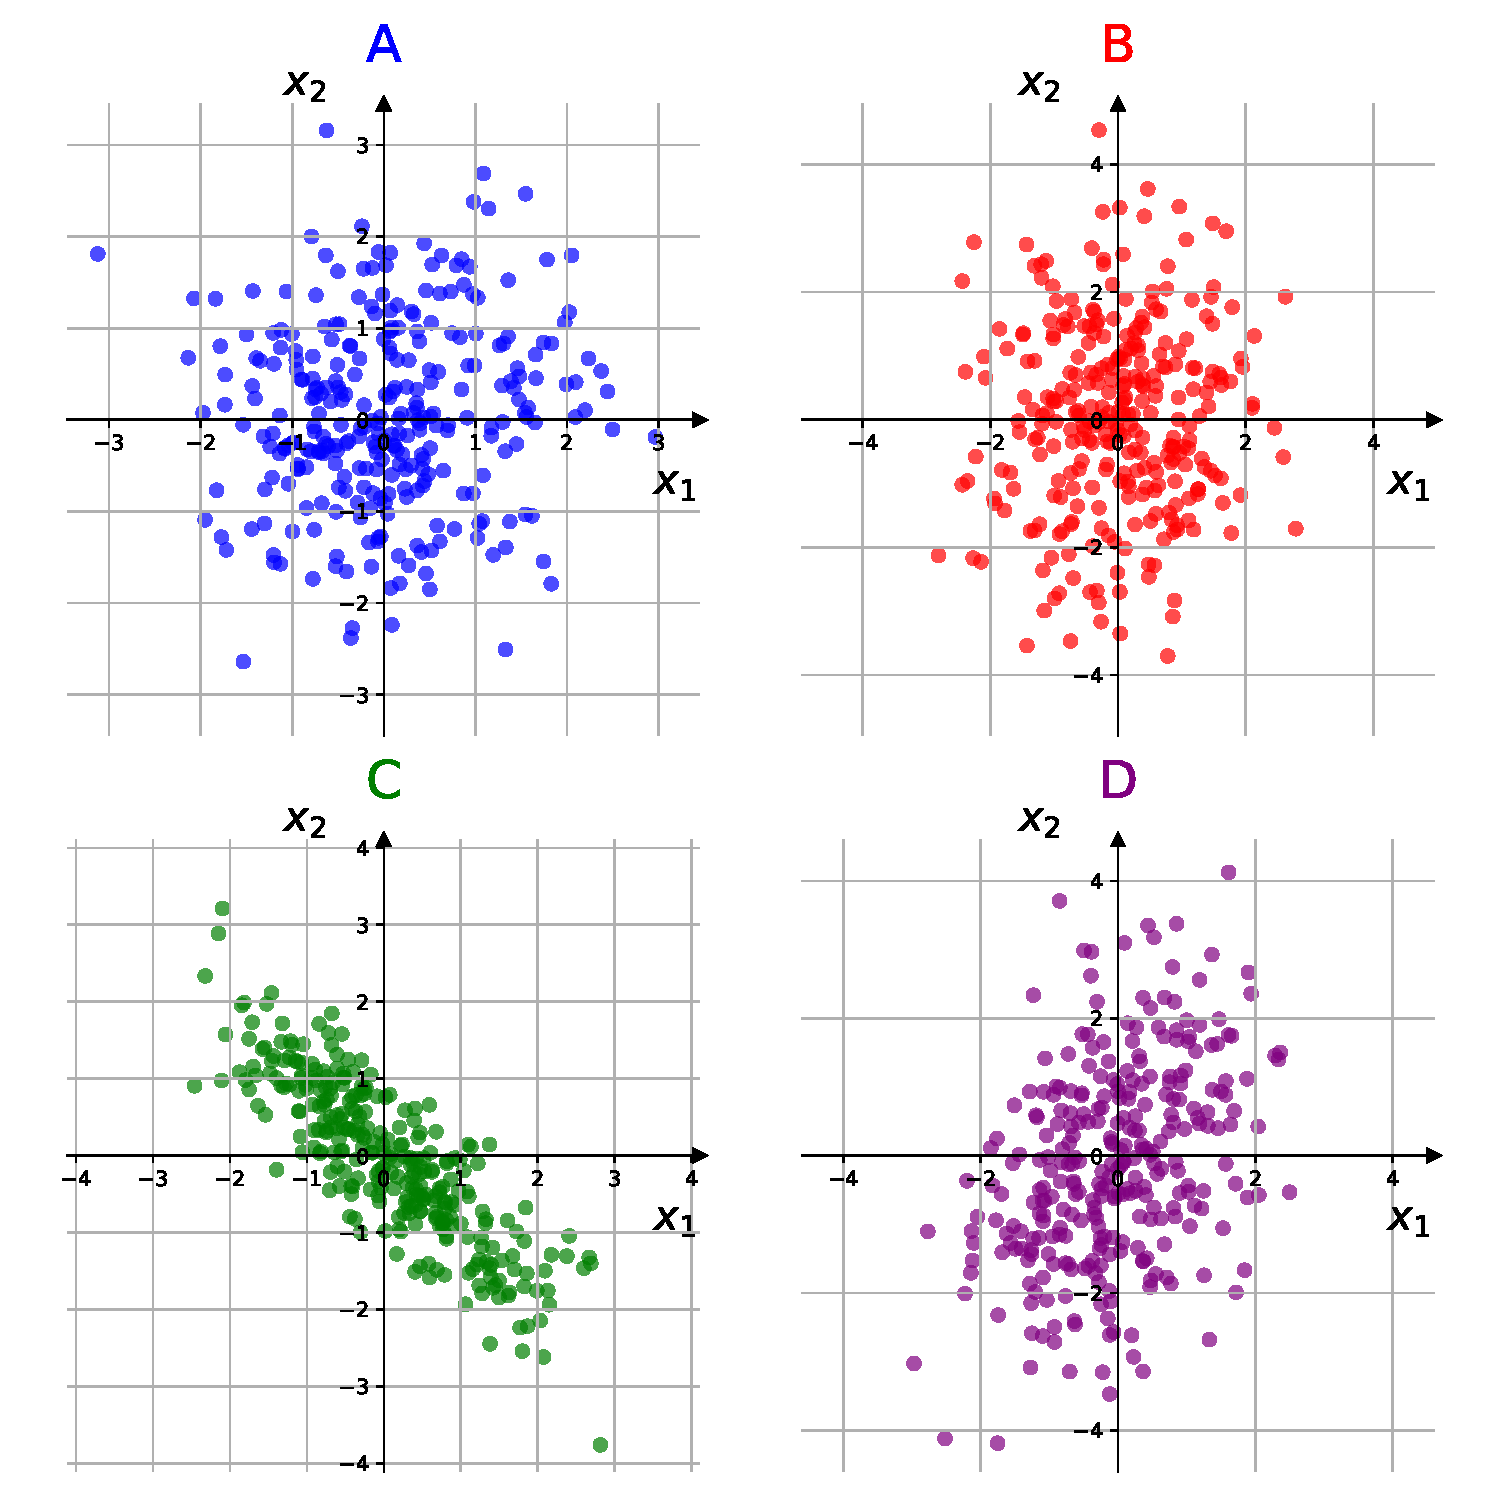
\includegraphics[width=0.55\textwidth]{img/scatter}%
\end{center}
}
\only<2>{
\begin{center}
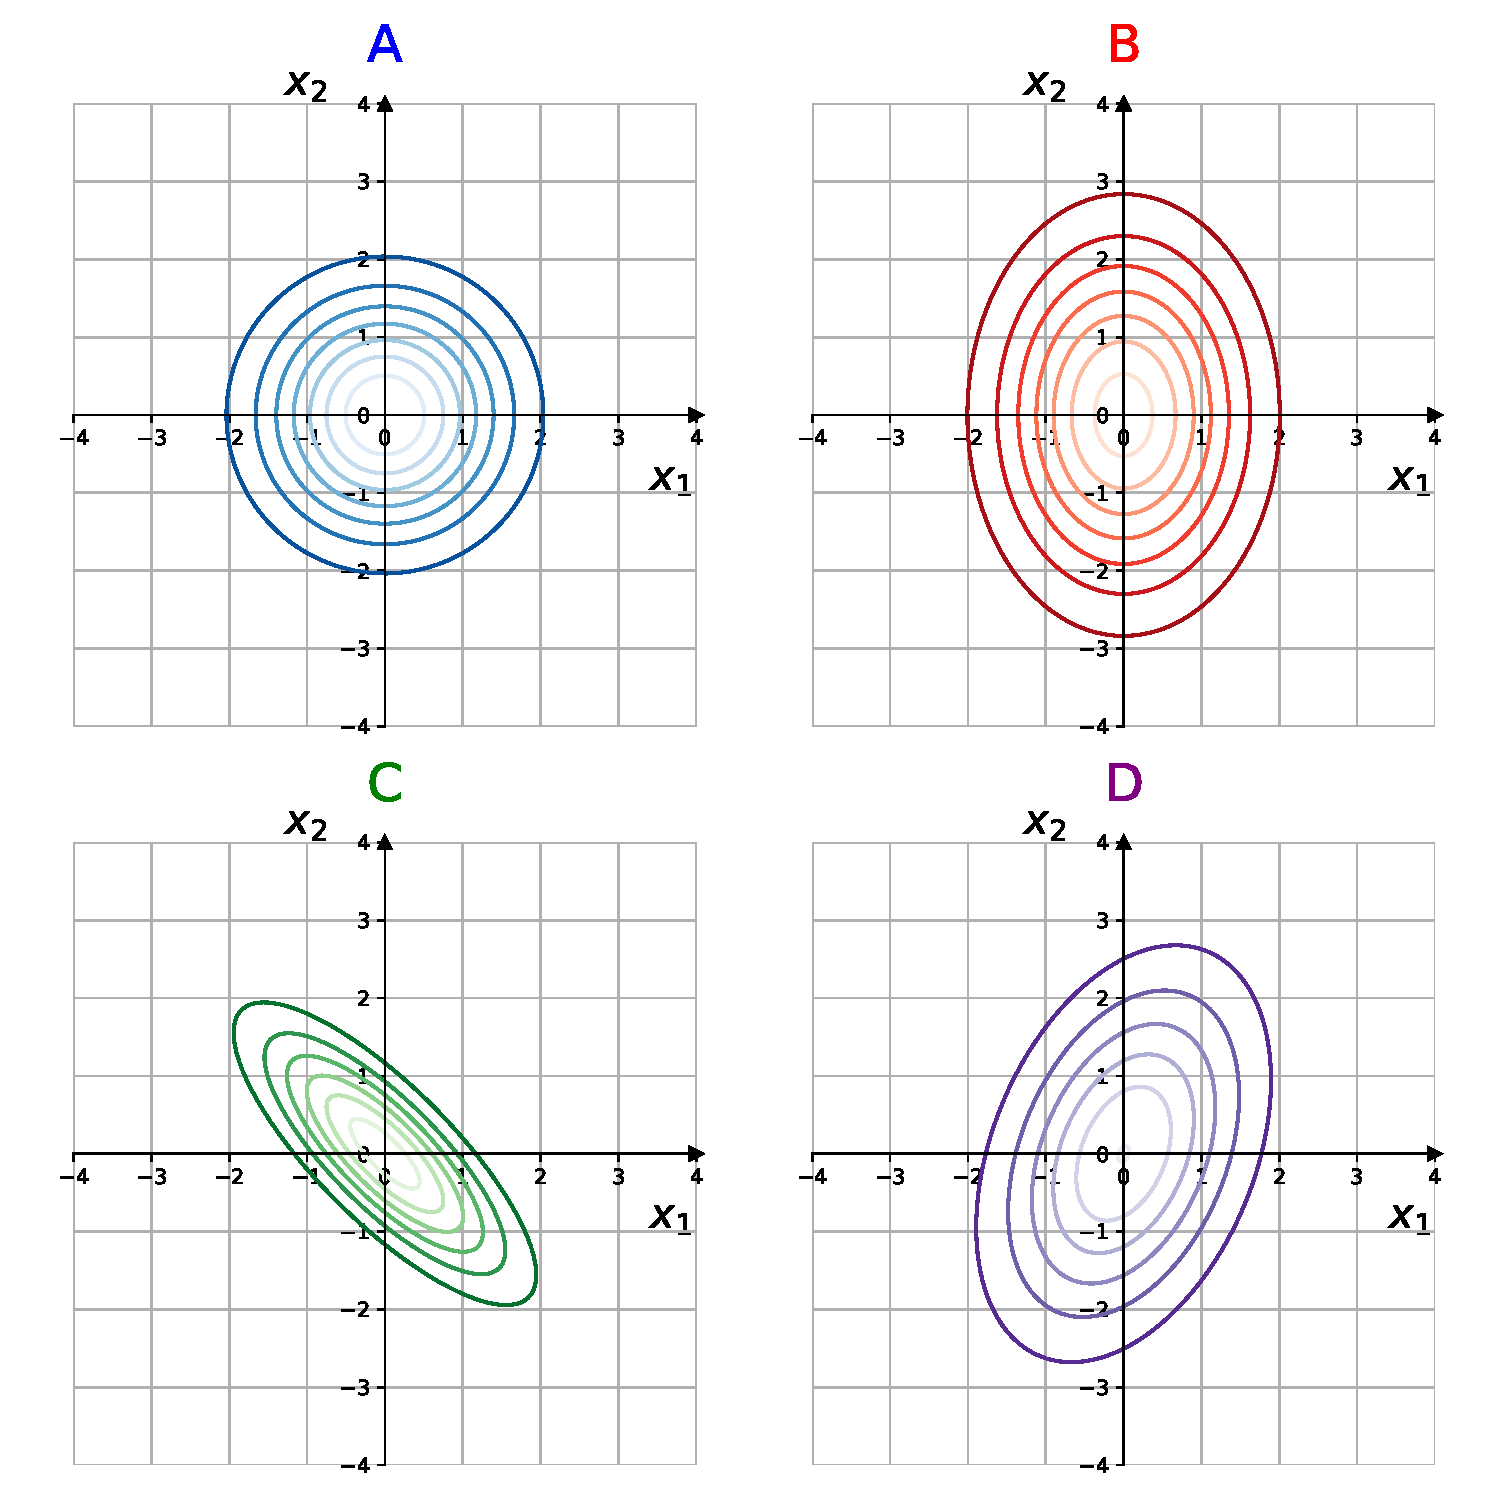
\includegraphics[width=0.55\textwidth]{img/cov}%
\end{center}
}

\svspace{-8mm}
}


\mode<article>{

\begin{figure}[ht]
     \centering
     \savebox{\imagebox}{
	 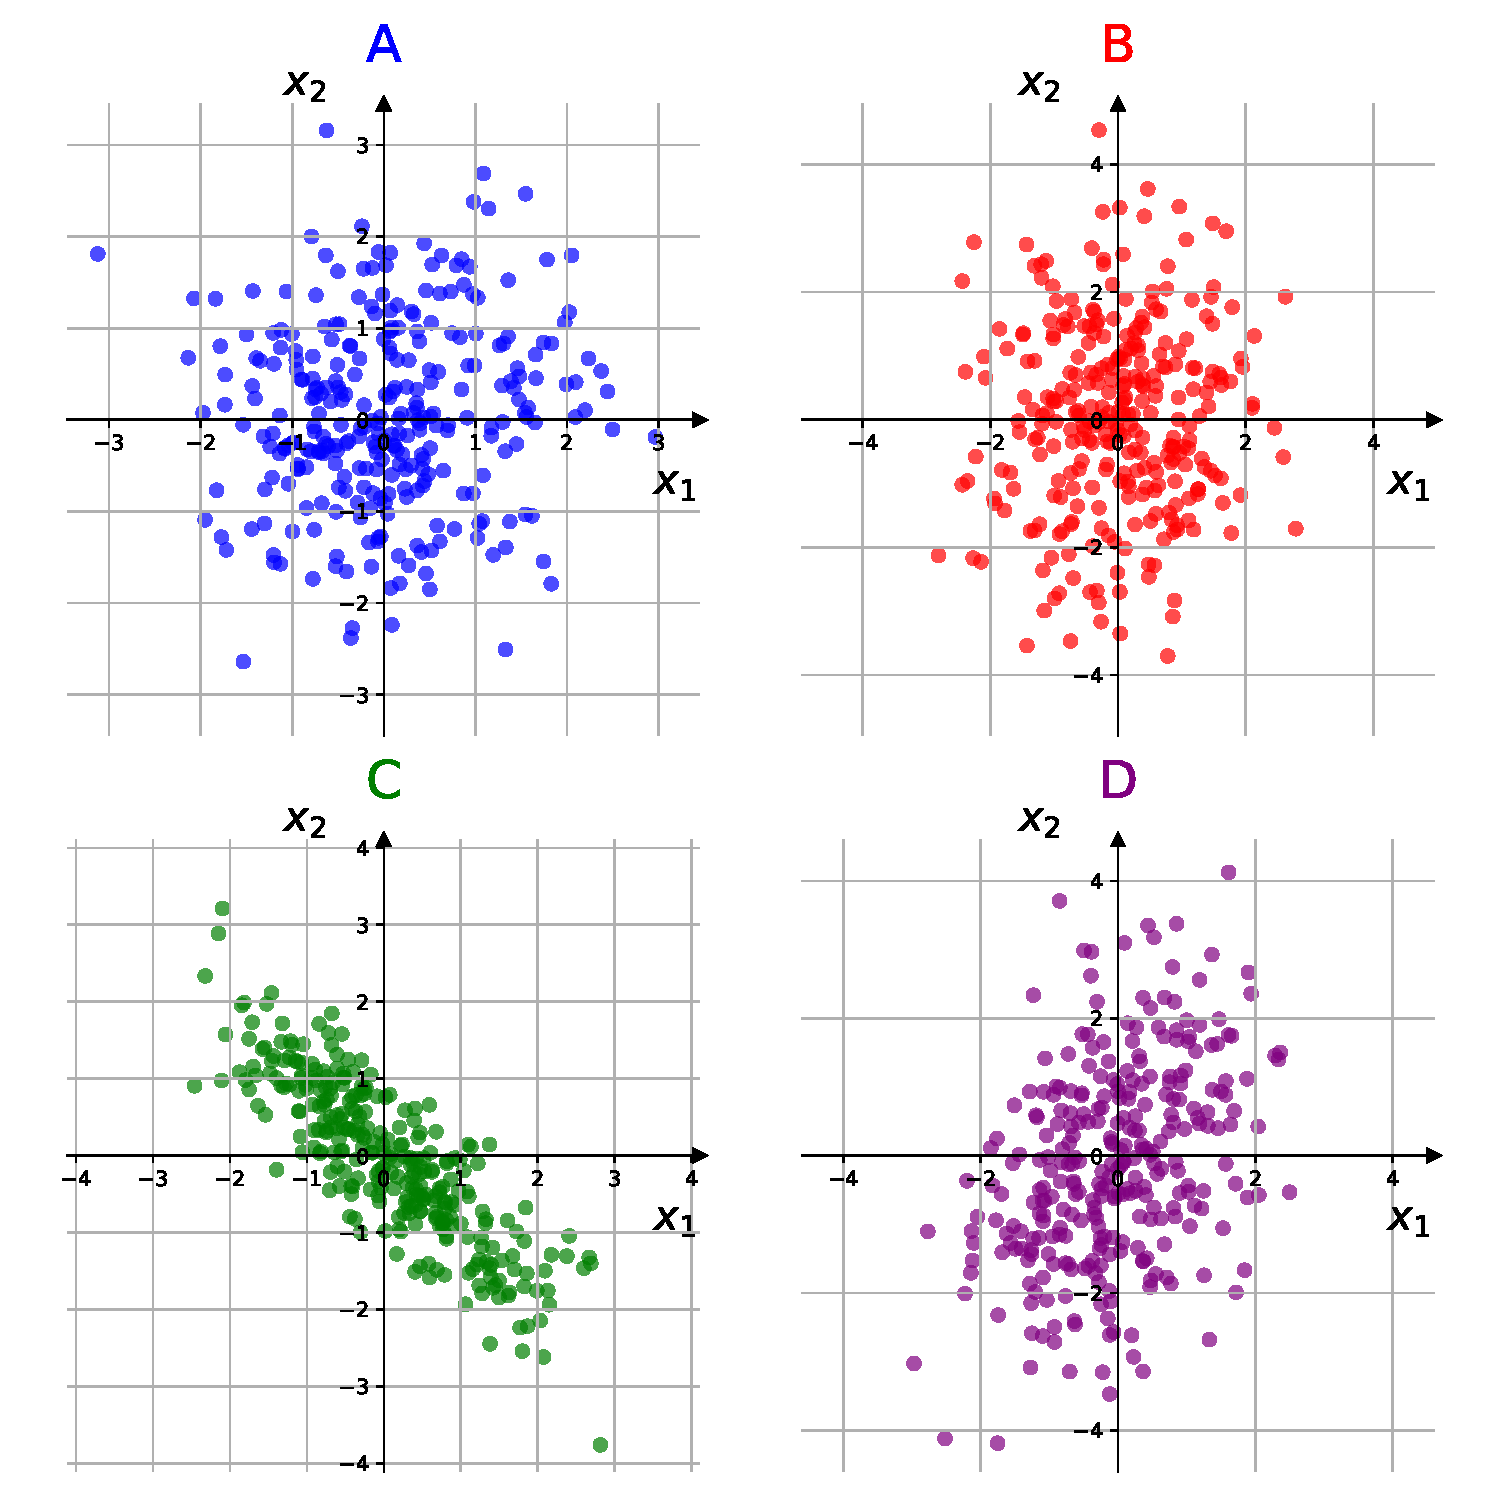
\includegraphics[width=0.33\textwidth]{img/scatter}}%
     \begin{subfigure}[t]{0.33\textwidth}
         \centering
         \usebox{\imagebox}% Place largest image
         \caption{Scatter plots}
     \end{subfigure}
     \hspace{2mm}
     \begin{subfigure}[t]{0.33\textwidth}
         \centering
         \raisebox{\dimexpr.5\ht\imagebox-.5\height}{% Raise smaller image into place
         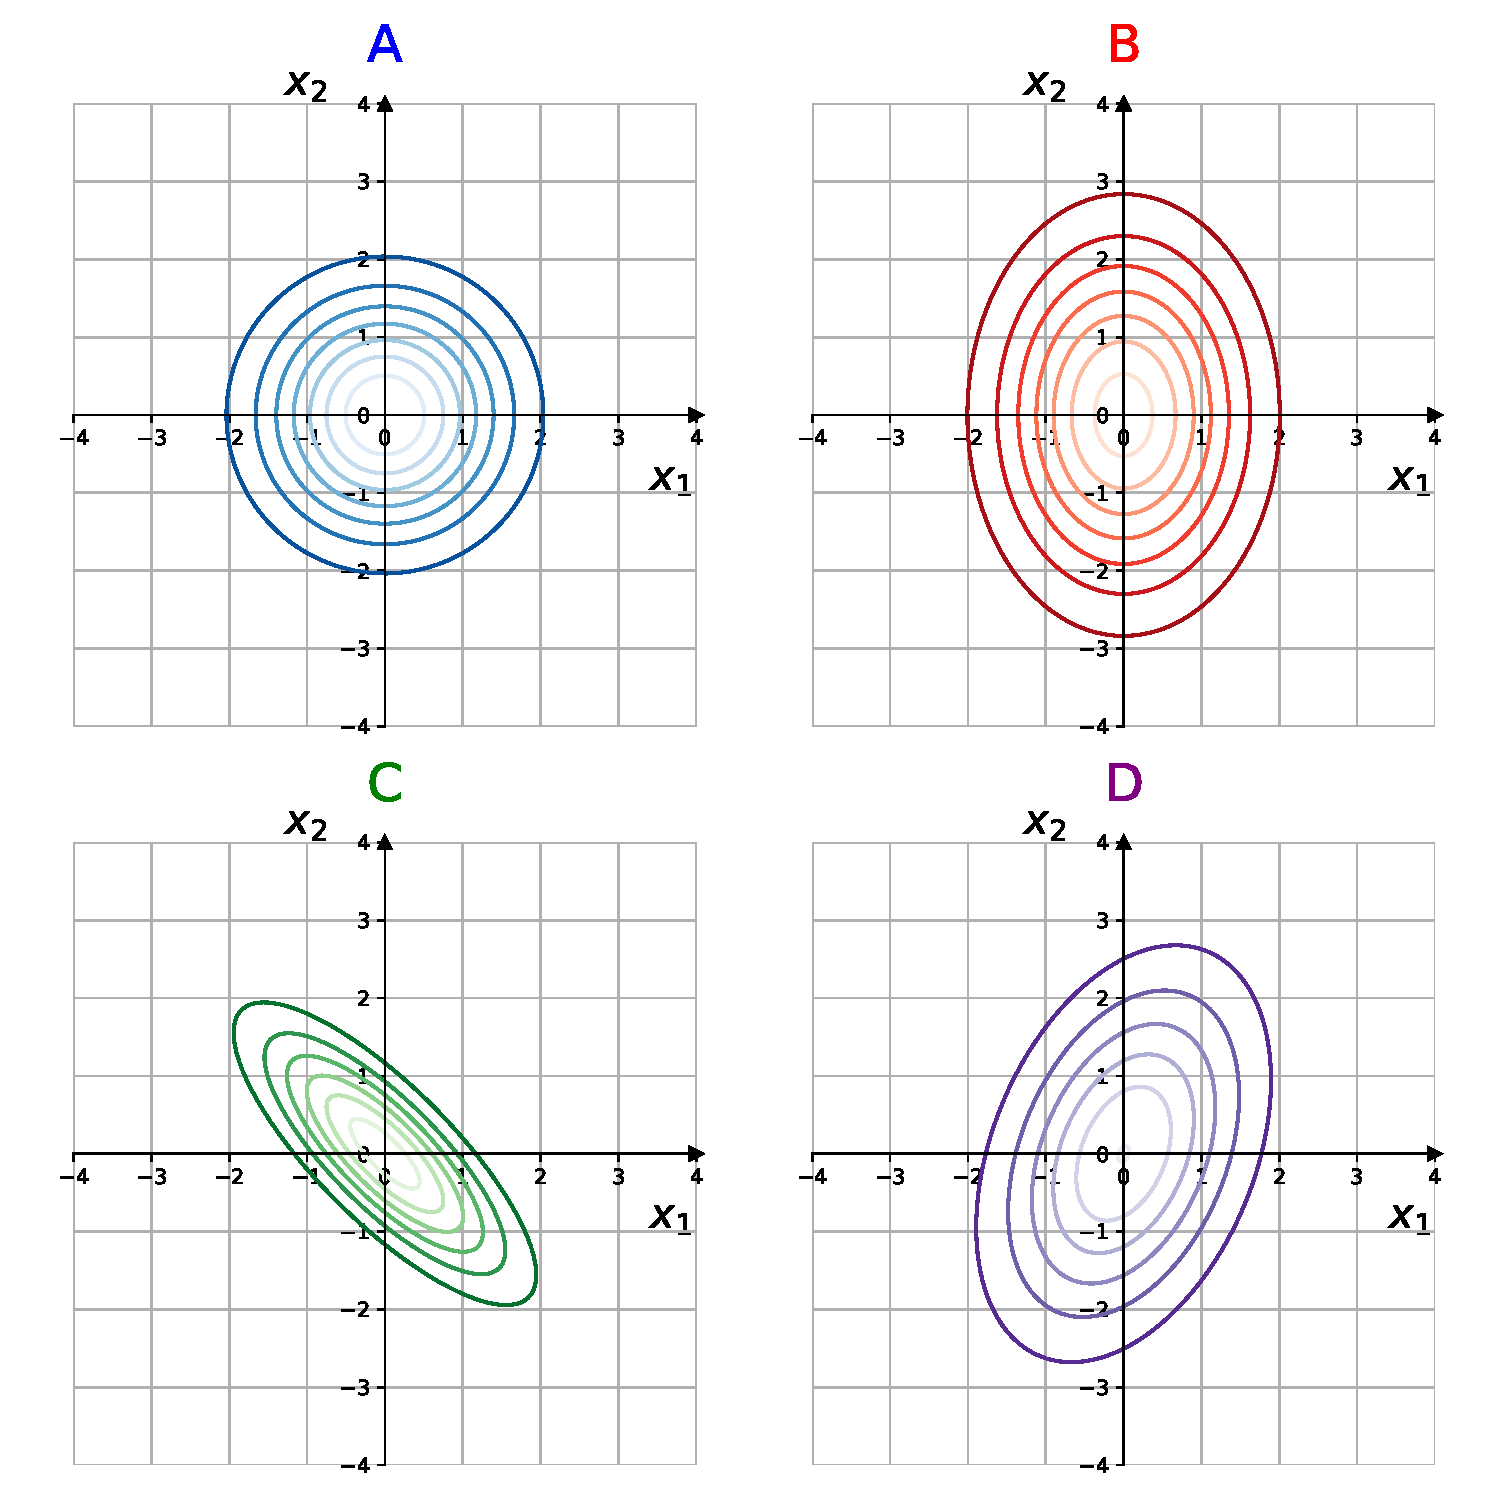
\includegraphics[width=0.99\textwidth]{img/cov}
         }
         \caption{Contour plots}
         \label{fig:linear}
     \end{subfigure}
\end{figure}
}

\question{Define a possible covariance matrix for each of the four datasets above.}

\mode<article>{

\begin{center}
\resizebox{.5\textwidth}{!}{%
\begin{tabular}{rl}
 ${\color{blue}\vec C_\mathrm{A} = \mat{1 & 0 \\ 0 & 1}}$ &  ${\color{red}\vec C_\mathrm{B} = \mat{1 & 0 \\ 0 & 2}}$\\[10mm]
 ${\color{darkgreen}\vec C_\mathrm{C} = \mat{1 & -0.8 \\ -0.8 & 1}}$ &  ${\color{byzantium}\vec C_\mathrm{D} = \mat{1 & 0.5 \\ 0.5 & 2}}$
\end{tabular}%
}
\end{center}
}



\end{frame}

\mode*

\clearpage

\mode<all>
\section{PCA}

\mode<presentation>{
\begin{frame} 
    \begin{center} \huge
        \secname
    \end{center}
    \begin{center}
    Transform and rotate the data s.t. keeping only the first $M$ dimensions has minimal MSE.
    \end{center}
\end{frame}
}

\subsection{Procedure and Projection}

\begin{frame}{Visible}\frametitle{\secname: \subsecname}

\begin{enumerate}
	\item<visible@1-> Center the data, $\E\lbrack\vec x\rbrack = \vec m  = \frac{1}{p} \sum_{\alpha=1}^{p} \vec x^{(\alpha)}\eqexcl \vec 0$.
\slidesonly{	\only<2>{
\svspace{5mm}
	\begin{center}
		\includegraphics[width=5cm]{img/meme_center}
    \end{center}
	}
}
	%\visible<3->
	%{
	\item<visible@3-> Let $\vec X$ be the $N \times p$ matrix of the centered data.
	\item<visible@4-> Measure
	\begin{itemize}
	\item the variance of each component in $\vec x$.\\
	\textbf{Not enough}, the variables in $\vec x$ could be correlated.
	\item the covariances $C_{ij} \;\; \forall\,i,j = 1,\ldots,N$.
	\item<visible@4->[$\Rightarrow$] Construct the covariance matrix $\vec C$.
		\begin{equation}
		\vec C = \text{Cov}(\vec X) = \mathbf{\Sigma} = \E\lbrack\vec X~\vec X^\top\rbrack \in \R^{N \times N}
		\end{equation}
	\end{itemize}
	\svspace{-5mm}
	\item<visible@6-> \textbf{eigenvalue decomposition}
	\item<visible@7-> Order eigenvalues in \emph{descending} order. (Highest variance first). The ordered eigenvectors are the \emph{principle components} of the dataset $\vec X$.
	\item<visible@8-> Project $\vec x$ onto the \textcolor{red}{first} $\color{red}M$ PCs.
	%}
\end{enumerate}


\end{frame}

\subsubsection{Eigenvalue decomposition}

\begin{frame}\frametitle{\subsubsecname}

\begin{equation}
\vec C \, \vec e_a \; = \; \lambda_a \vec e_a  \quad\text{(the eigenvalue problem of PCA)}
\end{equation}

\begin{itemize}
\item[] $\lambda_a: \text{the eigenvalue, the variance along principle component } a.$
\item[] $\vec e_a: \text{the \underline{normalized} eigenvector, the direction of the } a\text{-th PC in } \R^N$
\end{itemize}

\question{How do we perform an eigenvalue decomposition?}

\pause

\begin{enumerate}
\item Get eigenvalues:
\begin{equation}\det(\vec C-\lambda \vec I) = 0,
\end{equation} 
\item Find the eigenvector $\vec e_a$ associated with each $\lambda_a$ by solving the linear system
\footnote{If interested, see {\emph{math\_primer.pdf} on ISIS} for details and an example.}
\begin{equation}(\vec C - \lambda_a \vec I )\, \vec e_a = \vec 0
\end{equation}
\end{enumerate}

\end{frame}

\subsubsection{The Scree plot}

\begin{frame}\frametitle{\subsubsecname}

In PCA we sort the eigenvectors from highest to smallest eigenvalue.
Plotting the sorted eigenvalues is referred to as a \emph{scree plot}

\begin{center}
\includegraphics[width=0.6\textwidth]{img/screeplot_kpca_poly_d3}%
\captionof{figure}{Example of a scree plot}
\end{center}

\end{frame}

\subsubsection{Projection onto the PC space}

\begin{frame}\frametitle{\subsubsecname}

Recall \notesonly{from \sectionref{sec:objective} }that we wanted to \notesonly{improve on simple truncation by
transforming }\slidesonly{transform }the data before transmitting the first $M$ components.

\notesonly{We described the projection as follows:}

\begin{equation}
\vec u = \vec M^\top \vec x = (a_1,a_2,\ldots,a_N)^\top
\end{equation}


We can now define the transformation using the normalized eigenvectors of the PCs:

\begin{equation}
\vec M := (\vec e_1, \vec e_2, \ldots,\vec e_N)
\end{equation}

\slidesonly{

\begin{equation}
	\vec{x} = \underbrace{ a_1 }_{ \vec{e}_1^\top \vec{x} } \vec{e}_1
		+ \underbrace{ a_2 }_{ \vec{e}_2^\top \vec{x} } \vec{e}_2
		+ \ldots
		+ \underbrace{ a_N }_{ \vec{e}_N^\top \vec{x} } \vec{e}_N
\end{equation}
}


\end{frame}

\subsection{Reconstruction error}

\begin{frame}\frametitle{How much better is this vs. simple truncation of $\vec x$?}
%\newpage

\pause

\only<2,3>{
The transformation onto the PCs is linear:
\begin{equation}
	\vec{x} = \underbrace{ a_1 }_{ \vec{e}_1^\top \vec{x} } \vec{e}_1
		+ \underbrace{ a_2 }_{ \vec{e}_2^\top \vec{x} } \vec{e}_2
		+ \ldots
		+ \underbrace{ a_N }_{ \vec{e}_N^\top \vec{x} } \vec{e}_N
\end{equation}

Therefore, we can perfectly reconstruct observations by projecting them from PC space (i.e. feature space) back to the input space. \\
If we only use the \textcolor{red}{first} ${\color{red}M}$ PCs for reconstructing the observations, we will accumulate error.

\svspace{-5mm}

\begin{equation}
\widetilde{\vec{x}} = a_1 \vec{e}_1 + a_2 \vec{e}_2 + \ldots
		+ a_M \vec{e}_M
\end{equation}
}
		
\notesonly{We measure MSE between original centered observations and their corresponding reconstructions just as we did in \eqref{eq:mse}.}

\pause

\only<3,4>{
\begin{equation}
E = \frac{1}{p} \sum_{\alpha = 1}^{p} (\vec x - \widetilde{\vec x})^2 = \frac{1}{p} \sum_{\alpha = 1}^{p} \sum_{j = {\color{cyan}M+1}}^{{\color{cyan} N}} (a_j^{(\alpha)})^2
\end{equation}
}
\only<4>{
\svspace{5mm}

The MSE is equal to the sum of variances of the \textcolor{cyan}{last} $\notesonly{N-(M+1)-1=}{\color{cyan}N-M}$ components of the \emph{transformed} observations $\vec u=\vec M^\top \vec x$.\\

\svspace{5mm}

\notesonly{Since the PCs are ordered w.r.t to variance in descending order, }\notesonly{t}\slidesonly{T}he variances of the \textcolor{cyan}{last} $\color{cyan}N-M$ components of the transformed data are smallest.
The transformation is therefore optimal in the sense of minimal MSE.
}

\end{frame}

\mode*

%\clearpage

\mode<all>
\subsection{Applying PCA}

\mode<presentation>{
\begin{frame} 
    %\begin{center} \huge
        %\subsecname
    %\end{center}
    \begin{center}
		\includegraphics[width=5cm]{img/meme_knowpca}
    \end{center}
    \begin{center}What can we do with it?
    \end{center}
\end{frame}
}


\begin{frame}\frametitle{\subsecname}

\begin{enumerate}
\item Dimensionality reduction
\item Visualization (e.g. plot the projections onto the first 2 or 3 PCs.)
\item Outlier detection (project onto PCs with \emph{smallest} eigenvalues)
\item Whitening (i.e. decorrelate the data) - exploit that eigenvectors form an orthonormal basis.
\begin{equation}
\vec x_{whitened}^{(\alpha)} = \vec{\Lambda}^{-\frac{1}{2}}\vec{M}^\top\vec{x}^{(\alpha)}
\quad
\forall \alpha
\end{equation}

\question{What is the covariance of $\vec x_{whitened}$?}

\pause

- the Identity matrix.

\end{enumerate}

\end{frame}

\newpage


\subsubsection{A note on implementation}

\begin{frame}\frametitle{\subsubsecname}

\question{Is an off-the-shelf implementation such as\\ sklearn.decomposition.PCA for python really necessary?}

\notesonly{
PCA boils down to solving the eigenvalue problem.
We bascially need a routine with which to solve the eigenvalue problem. 
}
\pause
\slidesonly{
    \begin{center}
		\includegraphics[width=5cm]{img/meme_eig}
    \end{center}
    }
\pause

For python, the obvious choice is to use a routine like \textit{numpy.linalg.eig(A)}. \emph{Watch out for how to interpret the output.}

\end{frame}

\begin{frame}{Only}\frametitle{\subsubsecname}

\svspace{-5mm}

\question{Are there alternatives to eigenvalue decomposition?}

\notesonly{Yes, namely,}

\underline{Singular Value Decomposition (SVD)}:\\
Let $\vec X \in \R^{N \times p}$ be the centered dataset (centering is a must):
\begin{equation}
\vec X_{N \times p} = \vec U_{N \times N} \, \vec S_{N \times p} \, \vec V^\top_{{p \times p}}
\end{equation}
\svspace{-5mm}
where,
\begin{equation}
\vec U^\top \vec U = \vec I_{N \times N}
\notesonly{
\end{equation} and 
\begin{equation}
}
\slidesonly{\quad \text{and} \quad}
\vec V^\top \vec V = \vec I_{p \times p}
\end{equation} (i.e. $\vec U$, $\vec V$ are orthogonal).
\begin{itemize}

\item<only@2-> The columns of $\vec V$ (or rows of $\vec V^\top$) make up the eigenvectors of $\vec X^\top\vec X$.
\item<only@3-5> The columns of $\vec U$ make up the eigenvectors of $\vec X~\vec X^\top$.
\item<only@4,5> $\vec S$ is a diagonal matrix. The singular values in $\vec S$ (the diagonal entries) are the \textbf{square roots} of the  eigenvalues of the eigenvectors of $\vec X~\vec X^\top$ or $\vec X^\top\vec X$.
\end{itemize}

\only<5>{
Recall:
$$
\vec C = \E[\vec X~\vec X^\top] = \frac{1}{p} \vec X~\vec X^\top
$$
}

\end{frame}

\begin{frame}\frametitle{\subsubsecname}

\question{When to use \textit{SVD} vs. \textit{eig}? \textbf{Not dogma}}

\begin{itemize}

\item Numerical instabilities in eigendecomposition of very large covariance matrix $\rightarrow$ \textit{SVD}
\item \textit{SVD} is not applicable to Kernel-PCA $\rightarrow$ \textit{eig}
\item Computational efficiency $\rightarrow$ \textit{SVD} (depends...?)

\slidesonly{
$$
\vec X \in \R^{N \times p} \quad \leadsto \quad \vec C = \frac{1}{p} \vec X~\vec X^\top
$$
}
\item Possible differences between PCA via \textit{SVD} and PCA via \textit{eig}: \textit{SVD} may flip the sign.

\notesonly{

The reason for the difference in sign between the eigenvector's you would get via \textit{eig} and the eigenvector you would get via \textit{SVD}\footnote{Python's scikit-learn package uses SVD for its PCA implementation.}, is that SVD, in practice, may arbitrarily flip the direction of the eigenevectors.
Possible reasons for the sign ambiguity according to \cite{bro2008resolving}:
\begin{enumerate}
\item  It's a mechanism in the \textit{SVD} implementation (there's more than one \textit{SVD} implementation) to mitigate numerical instabilities,
\item Due to centering of the data,
\item an \textit{SVD} impelementation could have a random component.
\end{enumerate}

In both approaches you should be able to get the same reconstructions from both of them, i.e. the sign of the components along the flipped PC will also be flipped. Depending on the application, it may be necessary to ``detect'' if \textit{SVD} flipped the direction or not. Numerical methods to detect this exist. A reason to care about what the sign should be is when you want to interpret what an eigenvector represents to possibly assign meaning to the component along this PC: ``\textit{Is the component positive or negative along the PC or does this point have a larger component along the PC than another point?}''
The classical example of ``interpreting'' PCs would be ``Eigenfaces''. PCA is applied on images of faces. It is similar to what we ask you to do in Exercise 1.4. The Eigenvectors extracted from image data can be represented as images themselves. If \textit{SVD} gives you ``flipped'' eigenvectors, visualizing them would give you the ``negative'' of that image. It's not as intuitive to look at negatives, but a person will still be able to make sense of them. However, imagine trying to interpret the eigenvector of other high-dimensional data that isn't as pretty as pictures. Knowing that \textit{SVD} could have flipped the sign could give you a hard time trying to make sense of what the eigenvector represents.

}

\end{itemize}

\end{frame}


\mode*

\clearpage

\mode<article>{
\section{References}
\begin{frame}[allowframebreaks] \frametitle{References}
	\scriptsize
	\bibliographystyle{plainnat}
	\bibliography{bibliography}
\end{frame}
}

\end{rightcolumn}
\end{paracol}

\end{document}
